\chapter{Detailed Description}
\section{Interpreter}
\subsection{Introduction}
The interpreter is a complete implementation of an interpreter for the \mmc language. It accepts input from the parser in the form of an AST (\emph{Abstract Syntax Tree}) and obeys the instructions contained within the nodes of the tree. We call the tree traversal ``a tree walk" and we use this walk to interpret \verb!NODE! terms on the fly. We will see this kind of recursive pattern several times throughout the whole project.
\subsection{Initial Scan}
Firstly, the interpreter scans the AST, looking for global variables and function definitions. This initial scan is done, as we have no idea where to start interpreting without the presence of some kind of entry point into the user's code. It was decided that the most sensible approach would be to require the user-supplied definition of an \verb!int main(void)! entry-point function, in a similar vain to C. As this initial sweep of the AST takes place, any global variables or function declarations are entered into a structure known as the ``environment". 
\ \\ \ \\
Another benefit of performing this initial scan, is that as all outermost functions (and global variables) will now be entered into the environment. This means that functions may call other outer-level functions regardless of the order of definition (i.e if one function calls one which is declared lower down in the file). The same, however, does not apply to inner functions / variables.
\subsection{Environment}
Quite simply, the environment houses everything that the interpreter considers to be in local scope at a given execution point. As such, after our initial scan, we can detect the presence of a valid entry-point function by examining the environment. This initial environment is known as the ``global environment", as everything contained within, is visible to the whole user programme. This initial scan follows exactly the same code-path as the full interpreter does, but passes a flag, in order to ensure that function bodies are never stepped into.
\ \\ \ \\
The environment (depicted in figure \ref{fig:environment}) is a hash-table of \verb!values!. These values are references to inner functions or local variables. By following the static link between one environment and another (please see figure \ref{fig:environment}), it is possible to access and refer to values residing in outer scopes. The idea of a static link was given to us in relation to their use in Activation Records (please see section \ref{section:MIPS}) during lectures. Different information is stored for functions as opposed to variables. The \verb!value!'s type is determined with the following constants, the main types are given here, although there are some used for other purposes that are not mentioned here for the sake of clarity.

\begin{description}
	\item[VT\_INTEGR] Values of this type are integer variables, integer constants or integer temporaries.
	\item[VT\_STRING] Strings cannot be stored in the environment (this language does not have a string type), this value type is used to construct temporary strings that can be passed around within the interpreter / compiler. Such string values are created when identifiers are walked over, for instance.
	\item[VT\_FUNCTN] These values represent pointers to functions. This can be either a function variable or an actual function.
\end{description}

\subsection{Invoking the Entry Point}
If no entry point is found, a fatal error is raised as interpretation cannot continue without a valid entry point. If the entry point was found in our global environment, we lookup where the function definition was found in the AST and execute from this point. The \verb!environment.c! file gives us lots of useful search functionality in order to do things such as this. The particular search we do to find the main entry point is to look for a function in the global environment called \verb!main! with an integer return type and no formal parameters. If we get a match, we are returned a \verb!value! structure (of type \verb!VT_FUNCTN!) which meets our requirements within the global environment. These ``function values" each hold a reference to what \verb!NODE! in the AST is considered the ``start of the function". Once we have found the corresponding ``start of function" \verb!NODE! for the \verb!main()! function, we are able to continue the interpretation process by calling \verb!evaluate! on this entry \verb!NODE!.

\subsection{Recursive function - evaluate()}
The \verb!evaluate! function is now called recursively starting from the entry point. This scan is different from the initial scan, because we now look inside function bodies and any nested functions contained therein. Every time we enter a new function or block (such as an \emph{if statement} or \emph{while loop}), a new environment is created with a static link to the environment of the parent (enclosing) function (or the global environment, as appropriate). As we step over the tree in this recursive function, we encounter \verb!NODES! that are present in the AST. The following list mentions the steps that are taken for the several different (more interesting) types of node. The terms LHS and RHS refer to the \emph{left-hand side} and \emph{right-hand side} of an expression respectively. As the AST is a binary tree, the LHS and RHS can be thought of as the two child nodes under the current node. Please see figure \ref{fig:ast} for an example AST, that will use some of the elements mentioned below.

\begin{description}
	\item[Arithmetic Operator] We look at the LHS and RHS of the expression call \verb!evaluate! recursively on each. We do this, to try and simplify both sides (operands) into integers. From each recursive call we get back a \verb!value! typed struct for each, which should now contain our simplified integer. If one side happened to be a function application, for instance, the recursive call has already made the necessary calls to coerce this into the appropriate integer value. We calculate the result of the arithmetic expression and return the calculated value.
	\item[= Operator] This is the assignment operator. We call \verb!evaluate! on the LHS to get the variable into which the result will be stored. For the assignment to be valid, we must have already defined the assignment variable in the environment. Otherwise, we would be  using a variable that has not been declared yet. We call \verb!evaluate! on the RHS to find out the value that we're trying to assign to the variable on the LHS. Once we have the value back, we \textbf{type check} the assignment to ensure that the assignment is valid. This prevents the user making mistakes like trying to assign an integer to a function typed variable. The type checking operation is a simple check on the \verb!value! type on the LHS and RHS to check that they match. If the types do not match, then a fatal error describing the problem is raised. If all checks pass, then the existing LHS variable is updated with the new RHS value. This assignment will always affect the variable in the environment of its definition. The next time this LHS variable is referenced, it will have the newly assigned value.
	\item[APPLY] The \verb!APPLY! node type is encountered when a function call will occur. On the LHS of an \verb!APPLY! node is the function name identifier and the RHS contains the list of parameters that are being passed to the function. To invoke the function, the function name is searched for within the current environment (traversing static links where necessary). If a function typed variable is provided instead of a function application, this function variable holds enough information for us to invoke the function without having to traverse multiple levels of environment. If the function is \emph{still} not found, a fatal interpreter error is raised. If the function is found, we switch to the function's definition environment. In this environment, we store new variables with the formal parameter names, but with the specified parameter values used when calling the function. This assignment is also type checked with precisely the same method as before (see point ``\textbf{= Operator}" above). Once the checks are complete, we now pass the AST node representing the start of the function body to the \verb!evaluate! function and wait for control to return with the associated return value.
	\item[WHILE] While loops are also possible in \mmc. The implementation for a \verb!WHILE! statement within \mmc relies on the \verb!while! construct in the host development language (C). Inside the condition for the while loop, we recursively call \verb!evaluate! on the user specified condition. The condition is on the LHS of the \verb!WHILE! statement. In the body of our while loop, we call \verb!evaluate! on the RHS, which is the body of the user supplied while loop. The return value of the RHS evaluation is checked for several special cases. If we are returned the special \verb!$BREAK! or \verb!$CONTINUE! values then we \verb!break!, or \verb!continue! by using the  corresponding C keywords. If any other value is returned, we immediately exit the loop and return this value.
	\item[IF and ELSE] The \verb!IF! statement is fairly similar to the \verb!WHILE! statement in that the LHS holds the branch condition and we use C's \verb!IF! statement to implement it. Obviously the condition is only considered once in an \verb!IF! statement. One added complication with an if statement, is that an \verb!IF! can be followed by an \verb!ELSE! node. An \verb!ELSE! node needs access to the result of the \verb!IF! condition in order to decide whether to branch to the true or false part of the \verb!ELSE! (please see figure \ref{fig:if} for a graphical example). To get around this problem, when the condition is evaluated in the \verb!IF!, the result of that condition is placed into the environment as a temporary integer called \verb!$IF!. When the \verb!ELSE! statement executes, it checks the value of \verb!$IF! to see whether it should branch left or right.
	\item[Functions] Function definitions span multiple nodes in a tree, because of the amount of information that a function signature contains. Starting from higher up in the AST, we see nodes \verb!D, d, F!. The way each of these nodes is handled is mentioned below.
		\begin{description}
			\item[D] On the LHS is the \verb!d! node (explained below). On the RHS is the function body, i.e. the first instruction that constitutes the start of the used-defined function. Once we have evaluated \verb!d!, we store the returned value in the current environment along with a \textbf{reference} to the start of the function body. \verb!evaluate! is not called on the RHS, because this is only done when the function is called. The value returned by \verb!d! is a complete function definition that provides enough information for the declared function to be executed.
			\item[d] On the LHS is the return type of the function, this can be \verb!VOID, INT,! or \verb!FUNCTION!. We add the return type of the function into the temporary function variable returned by the \verb!F! node on the RHS. This is passed back up to the \verb!D! node ready to be stored in the environment.
			\item[F] On the LHS is the function name (identifier). On the RHS is the list of formal parameters. The interpreter calls \verb!evaluate! on the RHS with a special flag to denote any variables found as parameters, rather than normal variables. This call will return a linked list of \verb!value! structures which contains the parameter list. Once we have the function name and parameters, we build a temporary \verb!VT_FUNCTN value! structure, which will be gradually augmented with information as it is passed up to the \verb!D! node.
		\end{description}
	\item[RETURN] The value to return is found on the LHS of the \verb!RETURN! statement. \verb!evaluate! is called on the node to simplify arithmetic operations or the result of another function call. If the value to return is an identifier (i.e. a variable or a function ptr) then this is looked up in the environment and this \verb!value! (if found) is returned instead of the identifier. Additionally, we also type  check the return value by comparing the current function's return type to the value type of the evaluated return value. If the types match then the appropriate value is returned, otherwise a fatal error is raised. The same process prevents us returning \verb!NULL!, when a return value is expected (based on the function definition having a non-\verb!VOID! return type). \textbf{Please note:} there is no check to ensure that we actually use a return statement at all, where one is expected, only that - if we do use a return statement, it is type-checked.
\end{description}

\subsection{Returning from main()}
After traversing the AST, the \verb!main! function should have a valid integer return value (unless no \verb!RETURN! statement was present). This value is simply printed to standard out and the interpreter finishes.

\subsection{State of the Interpreter}
Within the limited time that we had for the whole project and the testing completed as part of this, the interpreter is seemingly complete. It is capable of executing all of the example scripts that I have created and there are no significant faults that I know of. There are two known faults that can be mentioned briefly.
\begin{itemize}
	\item One thing that does not work in the interpreter, but parses correctly: Functions without parameters that use the keyword \verb!void! to denote no parameters: \verb!int my_parameterless_fn(void)!.
	\item Return values are type-checked, but no effort is made to detect functions that do not return a value, when they should.
\end{itemize}

\begin{figure}[p]
	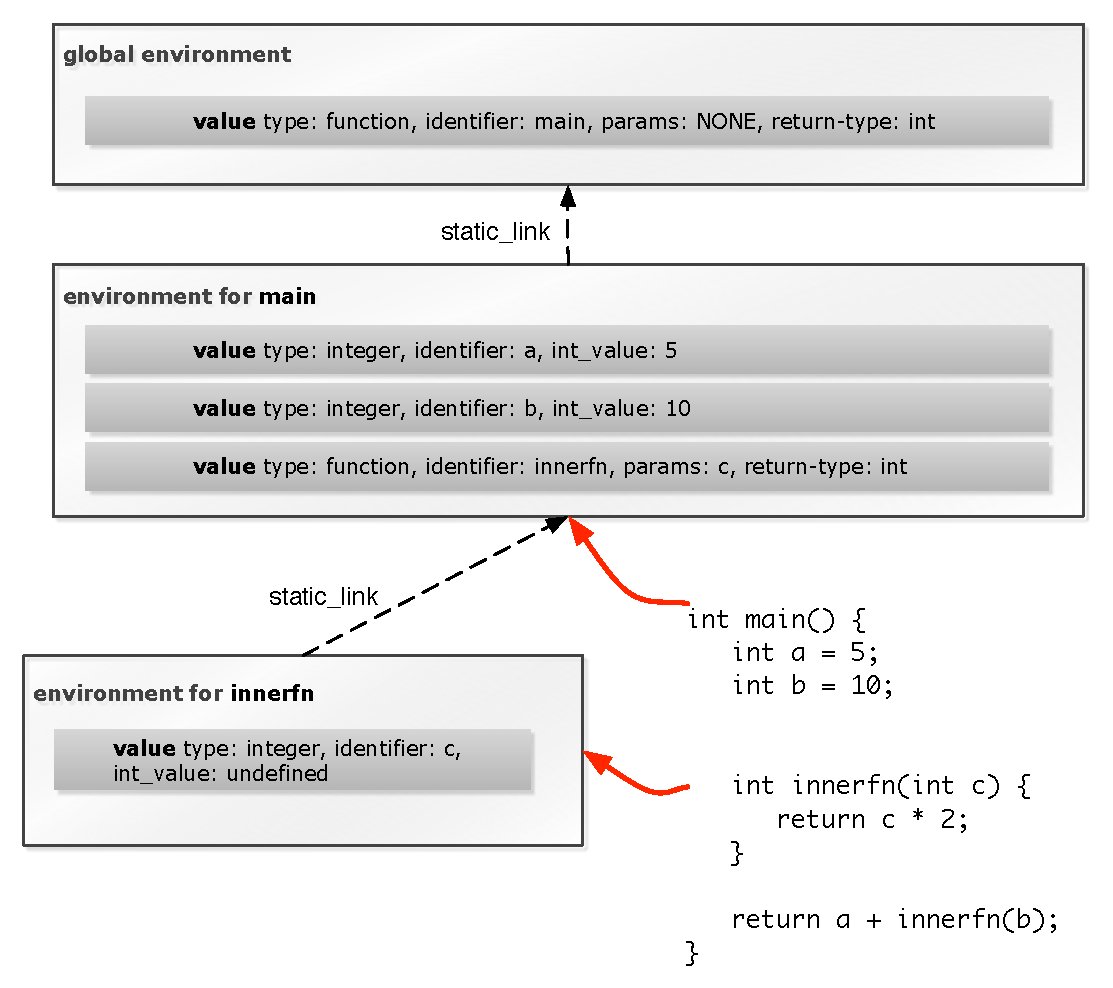
\includegraphics[scale=0.7]{environments-include.pdf}
	\caption{Environment Layout - Environment $\rightarrow$ Code relationship}
	\label{fig:environment}	
\end{figure}

\begin{figure}[p]
	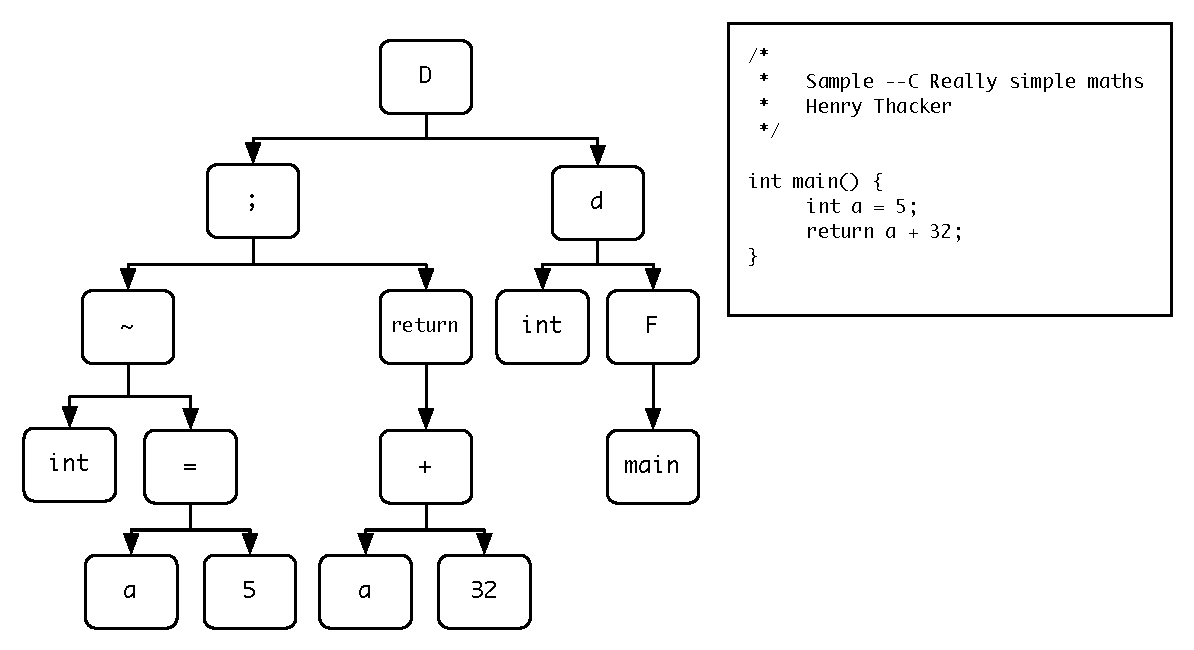
\includegraphics[scale=0.7]{ast-include.pdf}
	\caption{Abstract syntax tree example}
	\label{fig:ast}
\end{figure}

\begin{figure}[p]
	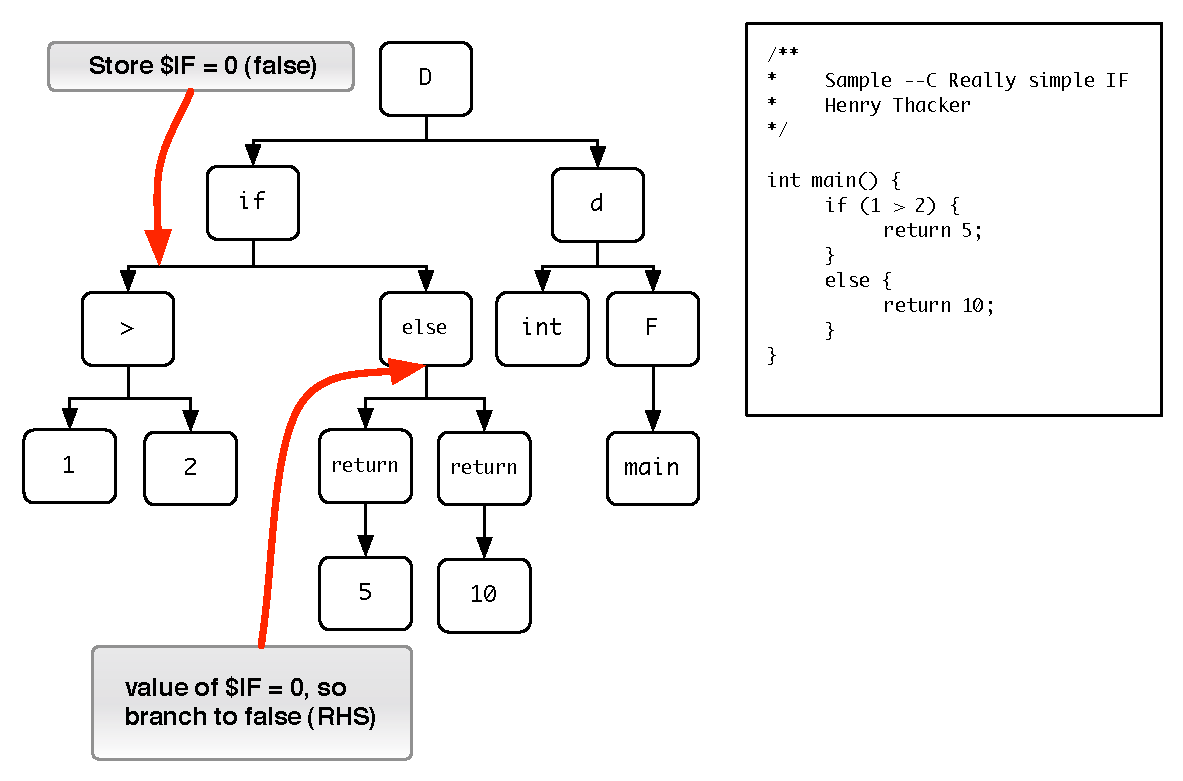
\includegraphics[scale=0.7]{if-include.pdf}
	\caption{IF, ELSE example}
	\label{fig:if}
\end{figure}

\begin{figure}[p]
	\begin{verbatim}
		typedef struct tac_quad {
		    char *op; /* Operation, i.e. + for addition */
		    value *operand1; /* A ptr to the first operand, could be an integer A */
		    value *operand2  /* A ptr to the first operand, could be an integer B */
		    value *result; /* The ptr to where the result will be stored, C */
		    int type; /* TT_OP - The type is an (arithmetic) operation */
		    int subtype; /* Reserved for categorisation of more granular operations */
		    int level; /* Used for MIPS code generation */
		    struct tac_quad *next; /* Pointer to the next tac_quad */		
		}tac_quad;
	\end{verbatim}
	\caption{tac\_quad structure}
	\label{fig:tacquad}
\end{figure}

\section{Intermediate Representation}

\subsection{Introduction}
In the coursework specification we were asked to develop a three address code representation of our own design. The input to the Three Address Code generator is the AST (\emph{Abstract Syntax tree}). The coursework specification indicates that it should be possible to read TAC (\emph{Three Address Code}) from a flat file. This was not implemented due to time pressures and it was felt that it was more important to move onto code generation, rather than write a TAC parser. The next section \ref{sec:tacintro} presents further background information behind the rationale of using a form of intermediate representation and the associated design choices that were made.

\subsection{Relation to the Interpreter}
The TAC is generated in a very similar way to how the interpreter works, using a large recursive function which handles all the different types of \verb!NODE!. Instead of evaluating the result of operations, we are interested in building TAC ``quadruples", internally referred to as a \verb!tac_quad!. Each \verb!tac_quad! is one TAC instruction and contains a \textbf{maximum} of three addresses (operand1, operand2, result) and several other pieces of metadata (please see figure \ref{fig:tacquad}). A \verb!tac_quad! does not contain text or lexemes, each address points to a \verb!value! within our environment. Thus, we are able to perform type checking and environment traversal, just as the interpreter does. The TAC generator generates a linked list of these \verb!tac_quad!s that represent the user-supplied \mmc source.
\ \\ \ \\
As with the interpreter, a pre-scan is done to find all function and variable names (in global scope) and everything is entered into the global environment. We still have to pre-scan, because when we look up variable and function names, we must be able to point our \verb!tac_quad!s to the correct references for them from an environment. No notion of an entry-point is required during TAC generation, because the AST is traversed in its entirety from top to bottom, generating \verb!tac_quad!s on the fly.

\subsection{Building tac\_quads}
After we have completed the pre-scan to populate our global environment, a full scan is made starting from the top of the AST. The TAC instructions are formed by examining each \verb!NODE! and evaluating the LHS and RHS until we have enough information to form a single, complete TAC instruction. The steps that are taken for a few different \verb!NODE! types are given below.

\begin{description}
	\item[Arithmetic Operator]
	\item[= Operator]
	\item[APPLY]
	\item[WHILE]
	\item[IF and ELSE]
	\item[Functions]
		\begin{description}
			\item[D]
			\item[d]
			\item[F]
		\end{description}
	\item[RETURN]
\end{description}

\section{MIPS Assembler Compiler}
\label{section:MIPS}